\documentclass[12pt,a4paper,oneside,openany]{book}

\usepackage{xcolor}
\usepackage{minted}
\usepackage[utf8]{inputenc}
\usepackage{tikz}
\usepackage{caption}
\usepackage{gensymb}
\usepackage{lmodern}
\usepackage{multirow}
\usepackage{booktabs}
\usepackage{array}
\usepackage{adjustbox}
\usepackage{upquote}
\usepackage{amsmath}
\usepackage{titlesec}
\usepackage[hidelinks]{hyperref}
\usepackage{fancyhdr}
\usetikzlibrary{mindmap,shadows, shapes, arrows, positioning}

%% Change these:
\newcommand{\projecttitle}{Unilodge \\[0.2cm] An AirBnB Service designed for students in the Galway area }
\newcommand{\projectauthor}{Aaron Burns \\[0.2cm] Faris Nassif}
\newcommand{\projectadvisor}{Dr. John French, Dr. Martin Kenirons}
\newcommand{\projectprogramme}{B.Sc.(Hons) in Software Development}
\newcommand{\projectdate}{\today}
%% End of things to change.



\tikzstyle{rect} = [rectangle, fill=blue!50, text width=4.5em, text centered, minimum height=4em, rounded corners]
\tikzstyle{line} = [draw, ->, very thick]
\tikzstyle{oval} = [ellipse, fill=green!50, text width=5em, text centered]

\newcolumntype{x}[1]{>{\centering\arraybackslash\hspace{0pt}}p{#1}}


\begin{document}
  \begin{titlepage}
    \begin{minipage}[t][6cm]{\textwidth}
      \centering
      \rule{\linewidth}{0.5mm} \\[0.4cm]
      { \LARGE \bfseries \projecttitle \\[0.4cm] }
      \rule{\linewidth}{0.5mm} \\[0.8cm]
    \end{minipage}
    
    \begin{minipage}[t][6.5cm]{\textwidth}
      \centering
      \textbf{\projectauthor}\\[0.5cm]
      \projectprogramme
    \end{minipage}
  
    \begin{minipage}[t][1cm]{\textwidth}
      \centering
      \textsc{\projectdate}
    \end{minipage}
      
    \begin{minipage}[t][3cm]{\textwidth}
      \centering
      \textbf{Unilodge}\\[0.3cm]
      Advised by: \projectadvisor \\[0.1cm]
      Department of Computer Science and Applied Physics\\
      Galway-Mayo Institute of Technology (GMIT)
    \end{minipage}
  
    \begin{center}    
      
\includegraphics{img/gmit-logo.jpg}
    \end{center}
  \end{titlepage}
  \setcounter{page}{2}
  \tableofcontents
  %!TEX root = project.tex

\chapter*{About this project}
\paragraph{Abstract}
This project is a rent hosting app akin to AirBnB except that is is exclusive for students in the Galway area (open to growth). It will allow users to create a hosting profile which allows them to let their properties to anyone else who is on the app. They can add some basic information about their property, anything a potential lodger would want to know. Such as price(and range), location, details, and a certain number of images of the property. Any other user of the site can view the profiles the user who created the profile page. The home page of the website will display an array of images for the user to see as soon as they log in. If they click on an image, they will be brought to the profile page to the that image comes from. 


\paragraph{Authors}
Aaron Burns, B.Sc.(Hons) in Software Development
Faris Nassif, B.Sc.(Hons) in Software Development

\chapter{Introduction}
From the moment we decided to do our project together, we knew that it would be best for us to develop a web application. This was something that over the past 3 years in this course we have become familiar with, but there was still a lot for both of us to learn. The first course of action was to decide what kind of application we wanted to build. It was difficult to get the ball rolling in terms of deciding what the app would actually do. From a number of projects in third year we had become familiar with CRUD operations (\textbf{Create, Read, Update, and Delete}). It was a basic essentially to this project that we at least implement CRUD, but that alone would only contribute to a small part of our project. We assumed for ourselves and were confirmed by our supervisors that CRUD functionally alone would be considered below the bare minimum needed for this \emph{Final Year Project}. In order for us to pass, and beyond that achieve a considerable mark in this module, we would need to expand on the knowledge we already have of \textbf{App Development} and implement some new technology or system that would show how we have learned something new in the course of creating this project. In order to meet this goal of self learning that was expected of us we knew that something we did would have to be at this moment in time completely new to us. However we would not feel confident jumping into all completely new technologies and languages just to meet this requirement. So we decided to complement the new materials we were going to learn with something that was familiar to us over our three year course.\newline\newline

\chapter{Context}
\begin{itemize}
\item Provide a context for your project.
\item Set out the objectives of the project
\item Briefly list each chapter / section and provide a 1-2 line description of what each section contains.
\item List the resource URL (GitHub address) for the project and provide a brief list of the main elements at the URL.
\end{itemize}

\section{Project Overview}
The initial idea for our project came from us meeting up and discussing ideas for an app that would be useful in the current climate of student accommodation being difficult to acquire. We did not have this plan going into these discussions, at first we had no clue what we could do with an app that would be considered clever or unique. It took us a time to arrive on our idea of a student lodging app for (at the moment) the Greater Galway area, and that came about from mulling over stories we had heard from our friends and issues we had heard 

\chapter{Methodology}
About one to two pages.
Describe the way you went about your project:
\begin{itemize}
\item Agile / incremental and iterative approach to development. Planning, meetings.
\item What about validation and testing? Junit or some other framework.
\item If team based, did you use GitHub during the development process.
\item Selection criteria for algorithms, languages, platforms and technologies.
\end{itemize}
Check out the nice graphs in Figure \ref{tikz:graphs}, and the nice diagram in Figure \ref{tikz:mydiagram}.

\begin{figure}
  \centering
  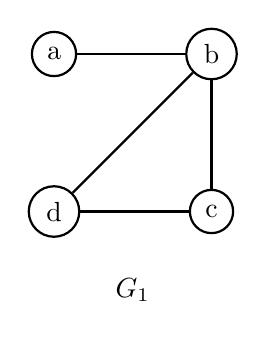
\begin{tikzpicture}
  \begin{scope}[every node/.style={circle,thick,draw}]
  \node (a) at (0,2) {a};
  \node (b) at (2,2) {b};
  \node (c) at (2,0) {c};
  \node (d) at (0,0) {d};
  \end{scope}
  \begin{scope}[every edge/.style={draw=black,thick}]
  \path (a) edge (b);
  \path (b) edge (c);
  \path (b) edge (d);
  \path (c) edge (d);
  \end{scope}
  \node () at (1,-1) {$G_1$};
  \end{tikzpicture}
  \hspace{1.5cm}
  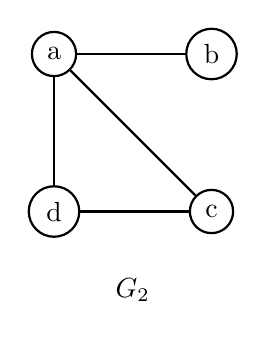
\begin{tikzpicture}
  \begin{scope}[every node/.style={circle,thick,draw}]
  \node (1) at (0,2) {a};
  \node (2) at (2,2) {b};
  \node (3) at (2,0) {c};
  \node (4) at (0,0) {d};
  \end{scope}
  \begin{scope}[every edge/.style={draw=black,thick}]
  \path (1) edge (2);
  \path (1) edge (3);
  \path (1) edge (4);
  \path (3) edge (4);
  \end{scope}
  \node () at (1,-1) {$G_2$};
  \end{tikzpicture}
  \caption{Nice pictures}
  \label{tikz:graphs}
\end{figure}
\section{Agile}
\section{Version Control}
\section{Testing}

\chapter{Technology Review}
About seven to ten pages.
\begin{itemize}
\item Describe each of the technologies you used at a conceptual level. Standards, Database Model (e.g. MongoDB, CouchDB), XMl, WSDL, JSON, JAXP.
\item Use references (IEEE format, e.g. [1]), Books, Papers, URLs (timestamp) – sources should be authoritative. 
\end{itemize}
\section{Vue}
\item Vue is a front-end web app development framework, similar to Angular and React. We considered using 
\sectiit wouon{Mon the ld fitgoDB}
\sVue as ection{Flask}
\section{Angular}
\section{Heroku}

\section{XML}
Here's some nicely formatted XML:
\begin{minted}{xml}
<this>
  <looks lookswhat="good">
    Good
  </looks>
</this>
\end{minted}

\begin{figure}
  \centering
  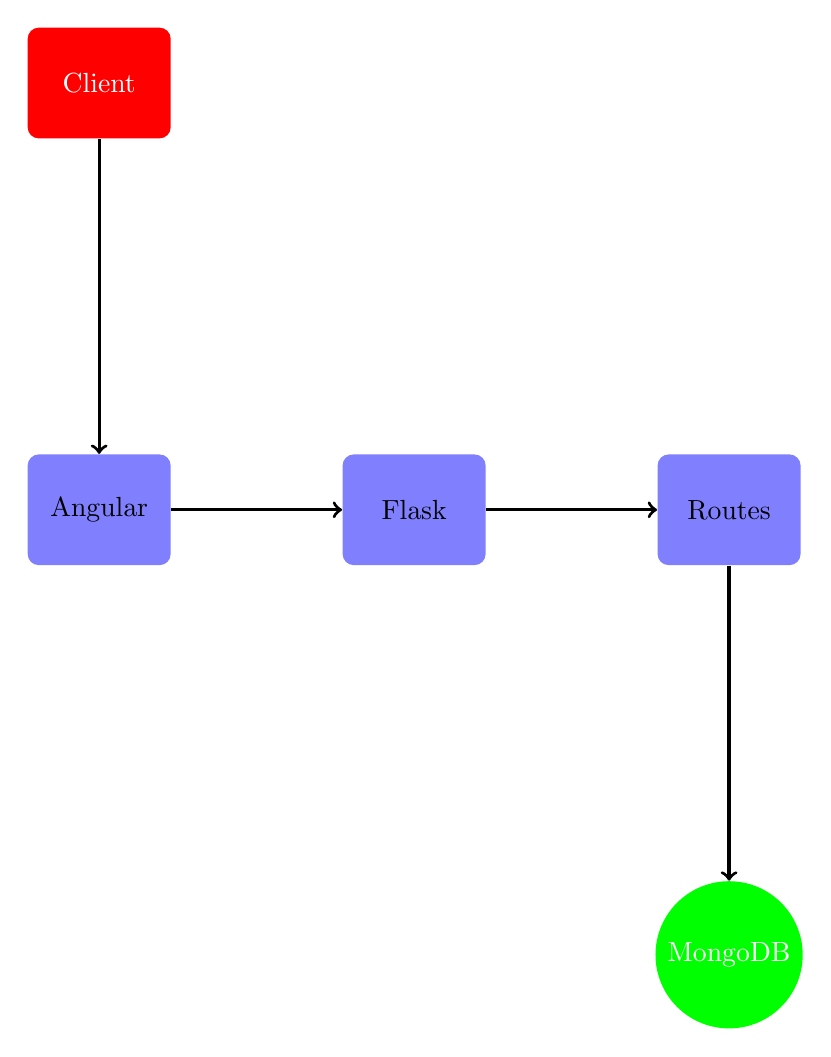
\begin{tikzpicture}[node distance=4cm]
  \node (a) [rect, fill=red, text=white] {Client};
  \node (b) [rect, below=of a] {Angular};
  \node (c) [rect, right of=b] {Flask};
  \node (d) [rect, right of=c] {Routes};
  \node (e) [circle, fill=green, text = white,  below=of d] {MongoDB};
  \draw [line] (a) -- (b);
  \draw [line] (b) -- (c);
  \draw [line] (c) -- (d);
  \draw [line] (d) -- (e);  
  \end{tikzpicture}
  \caption{Project Layout}
  \label{tikz:graphs}
\end{figure}

\chapter{System Design}
As many pages as needed.
\begin{itemize}
\item Architecture, UML etc. An overview of the different components of the system. Diagrams etc… Screen shots etc.
\end{itemize}

\begin{table}[h]
  \centering
  \begin{tabular}{x{2cm}p{3cm}}
    \toprule \\
    Column 1 & Column 2 \\
    \midrule \\
    Rows 2.1 & Row 2.2 \\
    \bottomrule
  \end{tabular}
  \caption{A table.}
  \label{table:mytable}
\end{table}

\chapter{System Evaluation}
As many pages as needed.
\begin{itemize}
\item Prove that your software is robust. How? Testing etc. 
\item Use performance benchmarks (space and time) if algorithmic.
\item Measure the outcomes / outputs of your system / software against the objectives from the Introduction.
\item Highlight any limitations or opportuni-ties in your approach or technologies used.
\end{itemize}

\chapter{Conclusion}
About three pages.

\begin{itemize}
\item Briefly summarise your context and objectives (a few lines).
\item Highlight your findings from the evaluation section / chapter and any opportunities identified.
\end{itemize}
  \bibliographystyle{ieeetr}
  \bibliography{bibliography}
\end{document}
